%%%%%%%%------------------------------------------------------------------------
% This program is free software: you can redistribute it and/or modify
% it under the terms of the GNU General Public License as published by
% the Free Software Foundation, either version 3 of the License, or
% (at your option) any later version.
% 
% This program is distributed in the hope that it will be useful,
% but WITHOUT ANY WARRANTY; without even the implied warranty of
% MERCHANTABILITY or FITNESS FOR A PARTICULAR PURPOSE.  See the
% GNU General Public License for more details.
% 
% You should have received a copy of the GNU General Public License
% along with this program.  If not, see <http://www.gnu.org/licenses/>.

%%%%%%%%------------------------------------------------------------------------
%%%% 导言区 
%% 文档类型为article
\documentclass[a4paper, 10pt]{book}
%1m = 39.4 inch
%大18开 (18.5cm * 23cm)
%\usepackage[left=3.25cm, right=3.25cm, top=2.3cm,bottom=1.4cm]{geometry}
\usepackage{geometry}
\geometry{left=3.75cm,right=3.25cm,top=3cm,bottom=2.5cm}

%% en_preamble包含基本的宏包配置
%%%%%%%%------------------------------------------------------------------------
%%%% 日常所用宏包

%%设置行间距
\usepackage{setspace}

%% 控制项目列表
\usepackage{enumerate}

%% 多栏显示
\usepackage{multicol}

%% hyperref宏包,生成可定位点击的超链接,并且会生成pdf书签
\usepackage[%
    pdfstartview=FitH,%
    CJKbookmarks=true,%
    bookmarks=true,%
    bookmarksnumbered=true,%
    bookmarksopen=true,%
    colorlinks=true,%
    citecolor=blue,%
    linkcolor=blue,%
    anchorcolor=green,%
    urlcolor=blue%
]{hyperref}

%% 控制标题
\usepackage{titlesec}

%% 控制表格样式
\usepackage{booktabs}

%% 控制目录
\usepackage{titletoc}

%% 控制字体大小
\usepackage{type1cm}

%% 首行缩进,用\noindent取消某段缩进
\usepackage{indentfirst}

%% 支持彩色文本、底色、文本框等
\usepackage{color,xcolor}

%% AMS LaTeX宏包
\usepackage{amsmath}
\usepackage{amssymb}

%% 一些特殊符号
% \usepackage{bbding}

%% 支持引用
% \usepackage{cite}

%% LaTeX一些特殊符号宏包
% \usepackage{latexsym}

%% 数学公式中的黑斜体
% \usepackage{bm}

%% 调整公式字体大小:\mathsmaller, \mathlarger
% \usepackage{relsize}

%% 生成索引
% \makeindex

%%%% 基本插图方法
%% 图形宏包
\usepackage{graphicx}
\usepackage{float}
%% 如果插入的图片没有指定扩展名,那么依次搜索下面的扩展名所对应的文件
\DeclareGraphicsExtensions{.pdf,.eps,.png,.jpg}
%% 让 latex 从 .bb 中读取 Bounding Box 信息
%\DeclareGraphicsRule{.jpg}{eps}{.bb}{}
%\DeclareGraphicsRule{.png}{eps}{.bb}{}
%\DeclareGraphicsRule{.pdf}{eps}{.bb}{}

%% 多个图形并排,参加lnotes.pdf
%\usepackage{subfig}
\usepackage{subfigure}


\usepackage{caption}
\captionsetup{font={sf, scriptsize}, labelfont={bf}, skip=15pt}
\DeclareCaptionLabelSeparator{colon}{~~}

\usepackage[perpage,stable]{footmisc}

\usepackage{longtable}
% \begin{figure}[htbp]               %% 控制插图位置
%   \setlength{\abovecaptionskip}{0pt}
%   \setlength{\belowcaptionskip}{10pt}
                                     %% 控制图形和上下文的距离
%   \centering                       %% 使图形居中显示
%   \includegraphics[width=0.8\textwidth]{CTeXLive2008.jpg}
                                     %% 控制图形显示宽度为0.8\textwidth
%   \caption{CTeXLive2008安装过程} \label{fig:CTeXLive2008}
                                     %% 图形题目和交叉引用标签
% \end{figure}
%%%% 基本插图方法结束

%%%% pgf/tikz绘图宏包设置
\usepackage{pgf,tikz}
\usetikzlibrary{shapes,automata,snakes,backgrounds,arrows}
\usetikzlibrary{mindmap, trees,  calendar}
\usetikzlibrary{positioning}
\usepackage{pgf-umlsd}
%% 可以直接在latex文档中使用graphviz/dot语言,
%% 也可以用dot2tex工具将dot文件转换成tex文件再include进来
%% \usepackage[shell,pgf,outputdir={docgraphs/}]{dot2texi}
%%%% pgf/tikz设置结束


%%%% fancyhdr设置页眉页脚
%% 页眉页脚宏包
\usepackage{fancyhdr}

%% 页眉页脚风格
\pagestyle{fancy}

%%这两行代码是修改\leftmark和\rightmark的经典模式
\renewcommand{\chaptermark}[1]{\markboth{{\hei {第\thechapter{}章}}\hspace 1  #1}{}}
\renewcommand{\sectionmark}[1]{\markright{\thesection{} #1}}

%% 清空当前页眉页脚的默认设置
\fancyhf{}

%\fancyhead[L]{\scriptsize \fangsong \ascii{ZTE}中兴}
%\fancyhead[R]{\scriptsize \fangsong 内部公开}

%\fancyhead[CE]{\scriptsize \fangsong \leftmark}
%\fancyhead[CO]{\scriptsize \fangsong \rightmark}

%\fancyfoot[RO, LE]{\scriptsize \thepage}
%\fancyfoot[C]{\scriptsize \fangsong 本文中的所有信息均为中兴通讯股份有限公司内部信息,不得向外传播}

\renewcommand{\headrulewidth}{0.4pt}
\renewcommand{\footrulewidth}{0.4pt}

%第{\couriernew\thechapter{}}章
%%下面开始修改页眉和页脚
\fancyhead[RE]{\fangsong \leftmark}
\fancyhead[LO]{\fangsong \rightmark}
\fancyhead[RO, LE]{\small \thepage}
\fancypagestyle{plain}{%
  \fancyhead{} % get rid of headers
  \renewcommand{\headrulewidth}{0pt} % and the line.
}

%%定义空白页面
\makeatletter
\def\cleardoublepage{\clearpage\if@twoside \ifodd\c@page\else
  \hbox{}
  \vspace*{\fill}
  \begin{center}
   {\sffamily\large}
   \end{center}
   \vspace{\fill}
   \thispagestyle{empty}
   \newpage
   \if@twocolumn\hbox{}\newpage\fi\fi\fi}
\makeatother

\makeatletter
\def\cleardedicatepage{\clearpage
  \hbox{}
  \vspace*{\fill}
  \begin{center}
   {\sffamily\Large 献给我的女儿刘楚溪}
   \end{center}
   \vspace{\fill}
   \thispagestyle{empty}
   \newpage
   \if@twocolumn\hbox{}\newpage\fi}
\makeatother

%% 有时会出现\headheight too small的warning
\setlength{\headheight}{15pt}
%%%% fancyhdr设置结束

%%设置行间距离
\usepackage{framed}  
%%%% listings宏包设置结束

%%%% 附录设置
\usepackage[title,titletoc,header]{appendix}
%%%% 附录设置结束

%%%% 日常宏包设置结束
%%%%%%%%------------------------------------------------------------------------

%%%%%%%%------------------------------------------------------------------------
%%%% 英文字体设置结束
%% 这里可以加入自己的英文字体设置
%%%%%%%%------------------------------------------------------------------------

%%%%%%%%------------------------------------------------------------------------
%%%% 设置常用字体字号,与MS Word相对应

%% 一号, 1.4倍行距
\newcommand{\yihao}{\fontsize{26pt}{36pt}\selectfont}
%% 二号, 1.25倍行距
\newcommand{\erhao}{\fontsize{22pt}{28pt}\selectfont}
%% 小二, 单倍行距
\newcommand{\xiaoer}{\fontsize{18pt}{18pt}\selectfont}
%% 三号, 1.5倍行距
\newcommand{\sanhao}{\fontsize{16pt}{24pt}\selectfont}
%% 小三, 1.5倍行距
\newcommand{\xiaosan}{\fontsize{15pt}{22pt}\selectfont}
%% 四号, 1.5倍行距
\newcommand{\sihao}{\fontsize{14pt}{21pt}\selectfont}
%% 半四, 1.5倍行距
\newcommand{\bansi}{\fontsize{13pt}{19.5pt}\selectfont}
%% 小四, 1.5倍行距
\newcommand{\xiaosi}{\fontsize{12pt}{18pt}\selectfont}
%% 大五, 单倍行距
\newcommand{\dawu}{\fontsize{11pt}{11pt}\selectfont}
%% 五号, 单倍行距
\newcommand{\wuhao}{\fontsize{10.5pt}{10.5pt}\selectfont}
%%%%%%%%------------------------------------------------------------------------

%%%%%%%%------------------------------------------------------------------------
%%%% 一些个性设置

%% 设定页码方式,包括arabic、roman等方式
%% \pagenumbering{arabic}

%% 有时LaTeX无从断行,产生overfull的错误,这条命令降低LaTeX断行标准
%% \sloppy

%% 设定目录显示深度\tableofcontents
%% \setcounter{tocdepth}{2}
%% 设定\listoftables显示深度
%% \setcounter{lotdepth}{2}
%% 设定\listoffigures显示深度
%% \setcounter{lofdepth}{2}

%% 中文破折号,据说来自清华模板
\newcommand{\pozhehao}{\kern0.3ex\rule[0.8ex]{2em}{0.1ex}\kern0.3ex}

%% 设定itemize环境item的符号
\renewcommand{\labelitemi}{$\bullet$}

%\makeatletter
%\@addtoreset{lstlisting}{section} 
%\makeatother

\newenvironment{enum}
{
  \begin{spacing}{1.2}
  \begin{enumerate}[1.]
    \setlength{\itemsep}{0pt} 
    \setlength{\itemindent}{2em}
    %\setlength{\listparindent}{2em}
}{%
  \end{enumerate}
  \end{spacing}
}

\newcommand{\suggest}[1]{
\tikzstyle{mybox} = [draw=black, very thick,
rectangle, rounded corners, inner sep=9pt, inner ysep=20pt]
\tikzstyle{fancytitle} =[fill=white, text=black, ellipse]
\noindent
\begin{tikzpicture}
\node [mybox] (box){%
\begin{minipage}{\textwidth}
\fangsong
#1
\end{minipage}
};
\node[fancytitle, right=10pt] at (box.north west) {\emph{建议}};
% \node[fancytitle, rounded corners] at (box.east) {$\clubsuit$};
\end{tikzpicture}
}

\newcommand{\notice}[1]{
\tikzstyle{mybox} = [draw=black, very thick,
rectangle, rounded corners, inner sep=9pt, inner ysep=20pt]
\tikzstyle{fancytitle} =[fill=white, text=black]
\noindent
\begin{tikzpicture}
\node [mybox] (box){%
\begin{minipage}{\textwidth}
\fangsong
#1
\end{minipage}
};
\node[fancytitle, right=10pt] at (box.north west) {\emph{注意}};
%\node[fancytitle, rounded corners] at (box.east) {$\clubsuit$};
\end{tikzpicture}
}

\newcommand{\tip}[1]{
\tikzstyle{mybox} = [draw=black, very thick,
rectangle, rounded corners, inner sep=9pt, inner ysep=20pt]
\tikzstyle{fancytitle} =[fill=white, text=black]
\noindent
\begin{tikzpicture}
\node [mybox] (box){%
\begin{minipage}{\textwidth}
\fangsong
#1
\end{minipage}
};
\node[fancytitle, right=10pt] at (box.north west) {\emph{提示}};
%\node[fancytitle, rounded corners] at (box.east) {$\clubsuit$};
\end{tikzpicture}
}

\newcommand\refch[1]{\ascii{第\ref{ch:#1}章(\nameref{ch:#1})}}
\newcommand\refsec[1]{\ascii{\ref{sec:#1}节(\nameref{sec:#1})}}

\newcommand\eitem[1]{\item {\itshape {#1}}}
\newcommand\cpp{\ascii{C\nobreak+\nobreak+}}
\newcommand\clang{\ascii{C}}
\newcommand\tf{\ascii{TensorFlow}}

\newcommand\quo[1]{“#1”}

\newcommand\percent[1]{\ascii{#1\%}}

\newcommand{\trans}{\emph{事务}}
\newcommand{\act}{\emph{操作}}
\newcommand{\seqact}{\emph{顺序操作}}
\newcommand{\conact}{\emph{并发操作}}
\newcommand{\atomact}{\emph{基本操作}}
\newcommand{\syncact}{\emph{同步操作}}
\newcommand{\asynact}{\emph{异步操作}}
\newcommand{\action}[1]{\emph{\ascii{\itshape\_\_#1}}}
\newcommand{\sigwait}{\action{sig\_wait}}
\newcommand{\sigsync}{\action{sig\_sync}}
\newcommand{\sigreply}{\action{sig\_reply}}
\newcommand{\timerprot}{\action{timer\_prot}}
\newcommand{\unknownevet}{\ascii{UNKNOWN\_EVENT}}
\newcommand{\transdsl}{\ascii{Transaction DSL}}
\newcommand{\oper}[1]{\ascii{Action#1}}
\newcommand{\protproc}{\ascii{prot\_procedure}}

%\newcommand{\code}[1]{\ascii{\small{\texttt{#1}}}}
\newcommand{\code}[1]{\ascii{\footnotesize{\texttt{#1}}}}

%\newcommand{\Email}{\begingroup \def\UrlLeft{<}\def\UrlRight{>} \urlstyle{tt}\Url}
%\def\mailto|#1|{\href{mailto:#1}{Email|#1|}}
\newcommand{\contrib}[2]{#1\quad{\small\quad\textit{#2}}\\[1ex]}
%% 设定正文字体大小
% \renewcommand{\normalsize}{\sihao}

%%%% 个性设置结束
%%%%%%%%------------------------------------------------------------------------


%%%%%%%%------------------------------------------------------------------------
%%%% bibtex设置

%% 设定参考文献显示风格

%%%% bibtex设置结束
%%%%%%%%------------------------------------------------------------------------


%% 如果不写中文的话就不需要引用xecjk_preamble里面的配置
%%%%%%%%------------------------------------------------------------------------
%%%% xeCJK相关宏包

\usepackage{xltxtra,fontspec,xunicode}

%% \CJKsetecglue{\hskip 0.15em plus 0.05em minus 0.05em}
%% slanfont: 允许斜体
%% boldfont: 允许粗体
%% CJKnormalspaces: 仅忽略汉字之间的空白,但保留中英文之间的空白。 
%% CJKchecksingle: 避免单个汉字单独占一行。
\usepackage[slantfont, boldfont]{xeCJK} 

%% 针对中文进行断行
\XeTeXlinebreaklocale "zh"             

%% 给予TeX断行一定自由度
\XeTeXlinebreakskip = 0pt plus 1pt minus 0.1pt

%%%% xeCJK设置结束                                       
%%%%%%%%------------------------------------------------------------------------

%%%%%%%%------------------------------------------------------------------------
%%%% xeCJK字体设置

%% 设置中文标点样式,支持quanjiao、banjiao、kaiming等多种方式
\punctstyle{quanjiao}                                        
                                                     
%% 设置缺省中文字体
\setCJKmainfont[BoldFont={Adobe Heiti Std}, ItalicFont={Adobe Kaiti Std}]{Adobe Song Std}   %  FZBaoSongZ04
%% 设置中文无衬线字体
\setCJKsansfont[BoldFont={Adobe Heiti Std}, ItalicFont={Adobe Kaiti Std}]{Adobe Kaiti Std}  
%% 设置等宽字体
\setCJKmonofont{Adobe Heiti Std}                            
%\setCJKmonofont{Monaco}                            

%% 英文衬线字体
\setmainfont{Lucida Bright}                                  
%% 英文等宽字体
%\setmonofont{Courier}
\setmonofont{Monaco}                             
%\setmonofont{Consolas}                              
%% 英文无衬线字体
\setsansfont{Optima}                                   

%% 定义新字体
\setCJKfamilyfont{song}{Adobe Song Std}                     
\setCJKfamilyfont{kai}{Adobe Kaiti Std}
\setCJKfamilyfont{hei}{Adobe Heiti Std}
\setCJKfamilyfont{fangsong}{Adobe Song Std}
\setCJKfamilyfont{lisu}{LiShu}
\setCJKfamilyfont{youyuan}{Adobe Kaiti Std}

%%自定义英文字体
\newfontfamily\couriernew{Lucida Grande}
\newfontfamily\optima{Optima}
\newfontfamily\lucida{Lucida Bright}

\newcommand{\ascii}[1]{{\sffamily #1}}
\newcommand{\speak}[1]{{\itshape #1}}
\renewcommand{\emph}[1]{{\hei #1}}

%% 自定义宋体
\newcommand{\song}{\CJKfamily{song}}                       
%% 自定义楷体
\newcommand{\kai}{\CJKfamily{kai}}                         
%% 自定义黑体
\newcommand{\hei}{\CJKfamily{hei}}                         
%% 自定义仿宋体
\newcommand{\fangsong}{\CJKfamily{fangsong}}               
%% 自定义隶书
\newcommand{\lisu}{\CJKfamily{lisu}}                       
%% 自定义幼圆
\newcommand{\youyuan}{\CJKfamily{youyuan}}                 

%%%% xeCJK字体设置结束
%%%%%%%%------------------------------------------------------------------------

%%%%%%%%------------------------------------------------------------------------
%%%% 一些关于中文文档的重定义

%% 数学公式定理的重定义

\newtheorem{example}{例}[section]                                   
\newtheorem{algorithm}{算法}
%% 按section编号
\newtheorem{theorem}{定理}[section]                         
\newtheorem{definition}{定义}
\newtheorem{axiom}{公理}
\newtheorem{property}{性质}
\newtheorem{proposition}{命题}
\newtheorem{lemma}{引理}
\newtheorem{corollary}{推论}
\newtheorem{condition}{条件}
\newtheorem{conclusion}{结论}
\newtheorem{assumption}{假设}

\newtheorem{principle}{原则}[section]
\newtheorem{regulation}{规则}[section]
\newtheorem{advise}{建议}[section]
\newtheorem{concept}{概念}[section]

%% 章节等名称重定义
\renewcommand{\contentsname}{目录}     
%\renewcommand{\abstractname}{摘要}
\renewcommand{\indexname}{索引}
\renewcommand{\listfigurename}{插图目录}
\renewcommand{\listtablename}{表格目录}
\renewcommand{\figurename}{图}
\renewcommand{\tablename}{表}
\renewcommand{\appendixname}{附录}
\renewcommand{\appendixpagename}{附录}
\renewcommand{\appendixtocname}{附录}
%\renewcommand\refname{参考文献} 

%%设置内容环境
\newenvironment{content}{%
  \setlength{\parskip}{0.5\baselineskip}
  \begin{spacing}{1.5}
}{%
  \end{spacing}
  \setlength{\parskip}{-0.5\baselineskip}
  \vskip -0.5\baselineskip
}

% 插入小段故事的语法:
% \begin{story}
%   \begin{center}
%     \inlinetitle{分水岭}
%   \end{center}
% \end{story}
\newenvironment{story}
{
  \setlength{\parskip}{0.5\baselineskip}
  \hbox to \textwidth{\hfil\rule{\linewidth}{0.5mm}\hfil}
  \begin{spacing}{1.5}
}{%
  \end{spacing}
  \hbox to \textwidth{\hfil\rule{\linewidth}{0.5mm}\hfil}
  \setlength{\parskip}{-0.5\baselineskip}
  \vskip -0.5\baselineskip
}

%% 设置chapter、section与subsection的格式
%\titleformat{\chapter}[display]{\flushright\yihao}{\thechapter{}}{1em}{\textbf}
\titleformat{\section}[block]{\flushleft\sanhao}{\optima{\thesection}}{1em}{\textbf}
\titleformat{\subsection}{\sihao}{\optima{\thesubsection}}{0.5em}{\textbf}
\titleformat{\subsubsection}{\xiaosi}{\thesubsubsection}{0.5em}{\textbf}

%\titlespacing{\chapter}{0pt}{0pt}{-\baselineskip}
\titlespacing{\section}{0pt}{0pt}{0\baselineskip}
\titlespacing{\subsection}{0pt}{0.5\baselineskip}{0\baselineskip}

%% 设置章格式
\usepackage{quotchap}

\renewcommand\chapterheadstartvskip{
   \vspace*{-5\baselineskip}
}

\renewcommand\chapterheadendvskip{
   \vspace*{0.5\baselineskip}
}

\usepackage{helvet}
\renewcommand\sectfont{\rmfamily\bfseries}

\newcommand\refig[1]{{\itshape \figurename\ascii{\ref{fig:#1}(第\pageref{fig:#1}页)}}}
\newcommand\reftbl[1]{{\itshape \tablename\ascii{\ref{tbl:#1}(第\pageref{tbl:#1}页)}}}

\renewcommand{\footnoterule}{\vspace*{3pt}%
  \hrule width 0.382\textwidth height 0.4pt \vspace*{2.6pt}}

% Remark
\newenvironment{remark}{\par\vskip10pt\footnotesize\itshape % Vertical white space above the remark and smaller font size
\begin{list}{}{
\leftmargin=35pt % Indentation on the left
\rightmargin=25pt}\item\ignorespaces % Indentation on the right
\makebox[-2.5pt]{\begin{tikzpicture}[overlay]
\node[draw=red!60,line width=1pt,circle,fill=red!25,font=\sffamily\bfseries,inner sep=2pt,outer sep=0pt] at (-15pt,0pt){\textcolor{red}{R}};\end{tikzpicture}}
\advance\baselineskip -1pt}{\end{list}\vskip5pt}

%%%% 中文重定义结束
%%%%%%%%------------------------------------------------------------------------


%%%% 设置listings宏包用来粘贴源代码
%% 方便粘贴源代码,部分代码高亮功能
\usepackage{listings}
\usepackage{color}

\DeclareCaptionFont{red}{\color{red}}

%% 所要粘贴代码的编程语言
\lstloadlanguages{{[LaTeX]TeX}, {[ISO]C++}, {Java}, {Ruby}, {Python}, {Scala}}

%% 设置listings宏包的一些全局样式
%% 参考http://hi.baidu.com/shawpinlee/blog/item/9ec431cbae28e41cbe09e6e4.html
\lstset{
numberbychapter=true,
breakatwhitespace=true,
showstringspaces=false,              %% 设定是否显示代码之间的空格符号
basicstyle=\footnotesize\ttfamily,           %% 设定字体大小\tiny, \scriptsize, \footnotesize, \small, \Large等等
keywordstyle=\bfseries,
commentstyle=\color{red!50!green!50!blue!50},                           
escapechar=`,                        %% 中文逃逸字符,用于中英混排
xleftmargin=1.5em,xrightmargin=0em, aboveskip=1em,
breaklines,                          %% 这条命令可以让LaTeX自动将长的代码行换行排版
extendedchars=false,                 %% 这一条命令可以解决代码跨页时,章节标题,页眉等汉字不显示的问题
frameround=fttt,
captionpos=top,
belowcaptionskip=1em
}

\lstdefinestyle{numbers}{
   numbers=left,
   numberstyle=\tiny,
   stepnumber=1,
   numbersep=1em
}

\lstdefinestyle{C++}{
   language=C++,
   texcl=true,
   prebreak=\textbackslash,
   breakindent=1em,
   keywordstyle=\bfseries, %% 关键字高亮
   morekeywords={alignas, alignof, char16_t, char32_t, constexpr, decltype, noexcept, nullptr, static_assert, thread_local, override, OVERRIDE, INTERFACE, ABSTRACT, DEFINE_ROLE, ROLE, HAS_ROLE, USE_ROLE}
   style=numbers,
   %frame=leftline,                     %% 给代码加框
   %framerule=2pt,
   %rulesep=5pt
}

\lstnewenvironment{c++}[1][]
  {\setstretch{1}
  \lstset{style=C++, #1}}
  {}

%\captionsetup[lstlisting]{textfont=red}
%{labelfont=bf, singlelinecheck=off, labelsep=space, textfont=red}

\lstdefinestyle{Java}{
   language=Java,
   texcl=true,
   prebreak=\textbackslash,
   breakindent=1em,
   keywordstyle=\bfseries, %% 关键字高亮
   morekeywords={}
   style=numbers,
   %frame=leftline,                     %% 给代码加框
   %framerule=2pt,
   %rulesep=5pt
}

\lstnewenvironment{java}[1][]
  {\setstretch{1}
  \lstset{style=Java, #1}}
  {}

\lstdefinestyle{Ruby}{
   language=Java,
   texcl=true,
   prebreak=\textbackslash,
   breakindent=1em,
   keywordstyle=\bfseries, %% 关键字高亮
   morekeywords={}
   style=numbers,
   %frame=leftline,                     %% 给代码加框
   %framerule=2pt,
   %rulesep=5pt
}

\lstnewenvironment{ruby}[1][]
  {\setstretch{1}
  \lstset{style=Ruby, #1}}
  {}

\lstdefinestyle{Python}{
   language=Python,
   texcl=true,
   prebreak=\textbackslash,
   breakindent=1em,
   keywordstyle=\bfseries, %% 关键字高亮
   morekeywords={}
   style=numbers,
   %frame=leftline,                     %% 给代码加框
   %framerule=2pt,
   %rulesep=5pt
}

\lstnewenvironment{python}[1][]
  {\setstretch{1}
  \lstset{style=Python, #1}}
  {}

\lstdefinestyle{Scala}{
   language=Scala,
   texcl=true,
   prebreak=\textbackslash,
   breakindent=1em,
   keywordstyle=\bfseries, %% 关键字高亮
   morekeywords={}
   style=numbers,
   %frame=leftline,                     %% 给代码加框
   %framerule=2pt,
   %rulesep=5pt
}

\lstnewenvironment{scala}[1][]
  {\setstretch{1}
  \lstset{style=Scala, #1}}
  {}  

\renewcommand{\lstlistingname}{示例代码}
\renewcommand\thefigure{\thechapter-\arabic{figure}}

\newcommand\refcode[1]{{\itshape \lstlistingname\ascii{\ref{code:#1}(第\pageref{code:#1}页)}}}


\usepackage[
  placement=center,
  angle=45,
  scale=4,
  color=black!40,
  %hshift=60,
  %vshift=-5
]{background}

\backgroundsetup{contents={TensorFlow Internals}}
%\backgroundsetup{contents={\includegraphics[width=0.2\textwidth]{figures/cock.jpg}}}

\newcommand{\myclearpage}{\clearpage{\pagestyle{empty}\cleardoublepage}}

%%%% 导言区结束
%%%%%%%%------------------------------------------------------------------------

%%%%%%%%------------------------------------------------------------------------
%%%% 正文部分

\begin{document}
\frontmatter
\pagestyle{empty}

%%自定义封面
\def\titlename{TensorFlow内核剖析}
\def\subtitle{TensorFlow Internals}
\def\authors{刘光聪}
\def\orgnization{\ascii{ZTE \textcopyright 2014}}


\newlength{\centeroffset}
\setlength{\centeroffset}{-0.5\oddsidemargin}
\addtolength{\centeroffset}{0.5\evensidemargin}
\thispagestyle{empty}

% \begin{tikzpicture}
%   \path[mindmap,concept color=black,text=white]
%     node[concept] {\ascii{Programming}}
%     [clockwise from=0]
%     child[concept color=green!50!black] {
%       node[concept] {\ascii{XP}}
%       [clockwise from=90]
%       child { node[concept] {\ascii{Simple Design}} }
%       child { node[concept] {\ascii{TDD}} }
%       child { node[concept] {\ascii{Refactoring}} }
%       child { node[concept] {\ascii{Pair Programming}} }
%     }
%     child[concept color=blue] {
%       node[concept] {\ascii{Oriented-Object}}
%       [clockwise from=-30]
%       child { node[concept] {\ascii{C++}} }
%       child { node[concept] {\ascii{Java}} }
%     }
%     child[concept color=red]
%     { node[concept] {\ascii{Evolutionary Design}} }
%     child[concept color=orange]
%     { node[concept] {\ascii{Clean Code}} };
%  \end{tikzpicture}

%title and subtitle
\vspace*{\stretch{1}}
\noindent\hspace*{\centeroffset}\makebox[0pt][l]{\begin{minipage}{\textwidth}
\flushright
{\Huge \hei \bfseries \titlename}
\noindent\rule[-1ex]{\textwidth}{5pt}\\[2.5ex]
\hfill\emph{\subtitle}
\end{minipage}}

%author
\vspace{\stretch{2}}
\noindent\hspace*{\centeroffset}\makebox[0pt][l]{\begin{minipage}{\textwidth}
\center
{\bfseries \authors} \\[1.5ex]
{\bfseries \orgnization}
\end{minipage}}

\vspace{\stretch{1}}

\pagebreak

\myclearpage

%\input{contents/foreword}
%\myclearpage

\chapter{前言} 
\label{ch:preface}

\section*{本书定位}

\begin{content}

这是一本剖析\ascii{TensorFlow}内核工作原理的书籍,并非讲述如何使用\ascii{TensorFlow}构建机器学习模型,也不会讲述应用\ascii{TensorFlow}的最佳实践。本书将通过剖析\ascii{TensorFlow}源代码的方式,揭示\ascii{TensorFlow}的系统架构、领域模型、工作原理、及其实现模式等相关内容,以便揭示内在的知识。

\end{content}


\section*{面向的读者}

\begin{content}

本书假设读者已经了解机器学习相关基本概念与理论,了解机器学习相关的基本方法论;同时,假设读者熟悉\ascii{Python, C++}等程序设计语言。

本书适合于渴望深入了解\ascii{TensorFlow}内核设计,期望改善\ascii{TensorFlow}系统设计和性能优化,及其探究\ascii{TensorFlow}关键技术的设计和实现的系统架构师、\ascii{AI}算法工程师、和\ascii{AI}软件工程师。

\end{content}

\section*{阅读方式}

\begin{content}

初次阅读本书,推荐循序渐进的阅读方式;对于高级用户,可以选择感兴趣的章节阅读。首次使用\ascii{TensorFlow}时,推荐从源代码完整地构建一次\ascii{TensorFlow},以便了解系统的构建方式,及其理顺所依赖的基本组件库。

另外,推荐使用\ascii{TensorFlow}亲自实践一些具体应用,以便加深对\ascii{TensorFlow}系统行为的认识和理解,熟悉常见\ascii{API}的使用方法和工作原理。强烈推荐阅读本书的同时,阅读\ascii{TensorFlow}关键代码;关于阅读代码的最佳实践,请查阅本书附录\ascii{A}的内容。

\end{content}

\section*{版本说明}

\begin{content}

本书写作时,\ascii{TensorFlow}稳定发布版本为\ascii{1.2}。不排除本书讲解的部分\ascii{API}将来被废弃,也不保证某些系统实现在未来版本发生变化,甚至被删除。

同时,为了更直接的阐述问题的本质,书中部分代码做了局部的重构;删除了部分异常处理分支,或日志打印,甚至是某些可选参数列表。但是,这样的局部重构,不会影响读者理解系统的主要行为特征,更有利于读者掌握系统的工作原理。

同时,为了简化计算图的表达,本书中的计算图并非来自\ascii{TensorBoard},而是采用简化了的,等价的图结构。同样地,简化了的图结构,也不会降低读者对真实图结构的认识和理解。

\end{content}

\section*{英语术语}

\begin{content}

因为我所撰写的文章,是供相关专业人士阅读,而非科普读物,因此在书中保留专业领域中朗朗上口的英语术语,故意不做翻译。例如,书中直接使用\ascii{OP}的术语,而不是将其翻译为「操作」。

但是,这会造成大面积的中英混杂的表达方式。幸运的是,绝对部分所使用的英语术语都是名词,极少出现动词或者形容词。但是,无论如何都不会丢失原本的主体语义和逻辑。

万事都有例外,对于无歧义的,表达简短,且语义明确的术语,会使用中文术语表示。特殊地,对于中文术语表达存在歧义时,会同时标注中文术语和英语术语。例如,检查点(\ascii{Checkpoint}),协调器(\ascii{Coordinator})。

一般地,无歧义的中文术语表定义在\reftbl{glossary}。

\begin{table}[!htb]
\resizebox{0.95\textwidth}{!} {
\begin{tabular*}{1.2\textwidth}{@{}ll@{}}
\toprule
\ascii{英文} & \ascii{中文} \\
\midrule
\ascii{Variable} & \ascii{变量,参数} \\
\ascii{Session} & \ascii{会话} \\ 
\ascii{Device} & \ascii{设备} \\ 
\bottomrule
\end{tabular*}
}
\caption{规范约定}
\label{tbl:glossary}
\end{table}

\end{content}

\section*{在线帮助}

\begin{content}

为了更好地与读者交流,在我的\ascii{Github}上建立了勘误表,及其相关补充说明。由于个人经验与能力有限,在有限的时间内难免犯错。如果读者在阅读过程中,如果发现相关错误,请帮忙提交\ascii{Pull Request},避免他人掉入相同的陷阱之中,让知识分享变得更加通畅,更加轻松,我将不甚感激。

同时,欢迎关注我的简书。我将持续更新相关的文章,与更多的朋友一起学习和进步。

\begin{enum}
  \eitem{\ascii{Github: \script{\url{https://github.com/horance-liu/tensorflow-internals-errors}}}}
  \eitem{\ascii{简书:\script{\url{http://www.jianshu.com/u/49d1f3b7049e}}}}
\end{enum}

\end{content}

\section*{致谢}

\begin{content}

感谢我的太太刘梅红,在工作之余完成对本书的审校,并提出了诸多修改的一件。

\end{content}

\myclearpage

\tableofcontents
\myclearpage

\def\thelstlisting{\thechapter-\arabic{lstlisting}}
%% 中文习惯是设定首行缩进为2em。
%% 注意此设置一定要在document环境之中,这可能与\setlength作用范围相关
\setlength{\parindent}{2em}

%%%%%%%%%%%%%%%%%%%%%%
%%开始正文,页面计数从正文开始
\mainmatter
\setcounter{page}{1}
\pagestyle{fancy}

\begin{savequote}[45mm]
\ascii{Any fool can write code that a computer can understand. Good programmers write code that humans can understand.}
\qauthor{\ascii{- Martin Flower}}
\end{savequote}

\chapter{介绍} 
\label{ch:introduction}

\begin{content}

\ascii{TensorFlow}是一个支持大规模和异构环境的机器学习系统。它使用数据流图\ascii{(Dataflow Graph)}表示计算过程和共享状态,使用节点表示抽象计算,使用边表示数据流。

数据流图的节点被映射在集群中的多个机器,在一个机器内被映射在多个计算设备\ascii{(Device)}上,包括\ascii{CPU, GPU, TPU}。\ascii{TensorFlow}灵活的架构支持多种计算平台,包括台式机,服务器,移动终端等。

\tf{}最初由\ascii{Google Brain}的研究员和工程师们开发出来,用于开展机器学习和深度神经网络方面的研究,但\tf{}优异的通用性使其也可广泛用于其他领域的数值计算。

\end{content}

\section{前世今生}

\begin{content}

\tf{}是\ascii{DistBelief}的后继者,它站在巨人的肩膀上,革命性地重新设计架构设计,使得\tf{}在机器学习领域一鸣惊人,在社区中产生了重大的影响。

为了更好地理解\tf{}系统架构的优越性,得先从\ascii{DistBelief}谈起。

\end{content}

\subsection{前世:DistBelief}

\begin{content}

\ascii{DistBelief}是一个用于训练大规模神经网络的的分布式系统,是\ascii{Google}第一代分布式机器学习框架。自\ascii{2011}年以来,在\ascii{Google}内部大量使用\ascii{DistBelief}训练大规模的神经网络。

\end{content}

\subsubsection{编程模型}

\begin{content}

\ascii{DistBelief}的编程模型是基于层\ascii{(Layer)}的\ascii{DAG(Directed Acyclic Graph)}图。层可以看做是一种组合多个运算操作符的复合运算符,它完成特定的计算任务。

例如,全连接层完成$f({W^T}x + b)$的复合计算,包括输入与权重的矩阵乘法,随后再与偏置相加,最后在线性加权值的基础上实施非线性变换。

\end{content}

\subsubsection{架构}

\begin{content}

\ascii{DistBelief}使用参数服务器\ascii{(Parameter Server)}的系统架构,训练作业包括两个分离的进程:无状态的\ascii{Worker}进程,用于模型训练的计算;有状态的\ascii{PS(Parameter Server)}进程,用于维护模型参数。

如\refig{parameter-server}所示,在分布式训练过程中,各个模型备份\ascii{(Model Relica)}异步地从\ascii{PS}上拉取\ascii{(Fetch)}训练参数$w$,当完成一步迭代运算后,推送\ascii{(Push)}参数的梯度$ \nabla w $到\ascii{PS}上去,并完成参数更新。

\begin{figure}[!htbp]
\centering
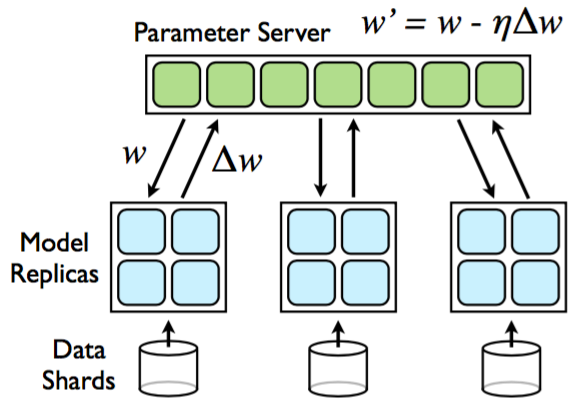
\includegraphics[width=0.6\textwidth]{figures/parameter-server.png}
\caption{DistBelief: Parameter Server架构}
 \label{fig:parameter-server}
\end{figure}

\end{content}

\subsubsection{缺陷与不足}

\begin{content}


但是,对于高级用户,\ascii{DistBelief}的编程模型,及其\ascii{Parameter Server}的系统架构,缺乏如下几个方面的扩展性。

\begin{enum}
  \eitem{优化算法:添加新的优化算法,必须修改\ascii{Parameter Server}的实现;\code{get(), put()}的抽象方法,对某些优化算法并不高效;}
  \eitem{训练算法:支持非前馈的神经网络具有很大的挑战性,例如包含循环的\ascii{RNN},交替训练的对抗网络,及其损失函数由分离的代理完成增强学习模型;} 
  \eitem{加速设备:\ascii{DistBelief}设计之初仅支持多核\ascii{CPU},并不支持\ascii{GPU};遗留的系统架构对支持新的计算设备缺乏弹性空间。}
\end{enum}

\end{content}

\subsection{今生:TensorFlow}

\begin{content}

正因为\ascii{DistBelief}遗留的架构和设计,不再满足潜在的深度学习与日俱增的需求,\ascii{Google}毅然决定在\ascii{DistBelief}基础上做全新的架构设计,从而诞生了\ascii{TensorFlow}。

\end{content}

\subsubsection{编程模型}

\begin{content}

\ascii{TensorFlow}使用数据流图\ascii{(Dataflow Graph)}表示计算过程和共享状态,使用节点表示抽象计算,使用边表示数据流。如\refig{tf-dataflow}所示,展示了\ascii{mnist}手写识别应用的数据流图。

在该模型中,前向子图使用了\ascii{2}层全连接网络,分别为\ascii{ReLU}层和\ascii{Softmax}层;随后,由\ascii{Gradients}构建了与前向子图对应的反向子图,用于训练参数的梯度计算;最后,使用`SGD`的优化算法,构造参数更新子图,完成参数的更新。

\begin{figure}[!htbp]
\centering
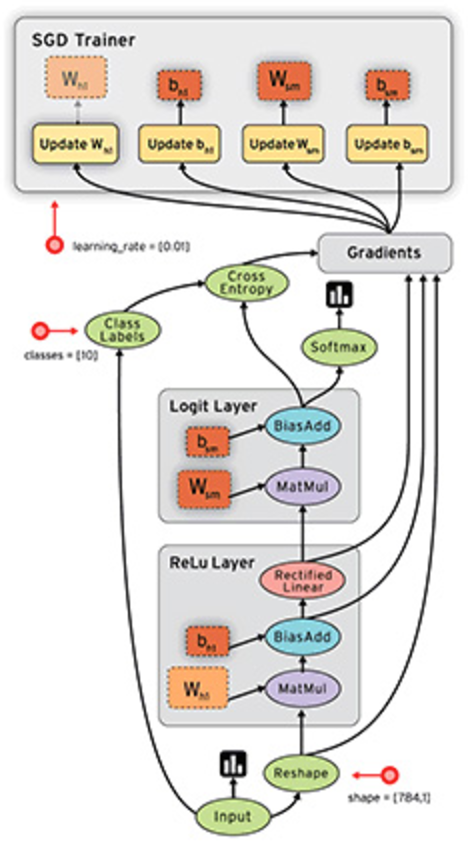
\includegraphics[width=0.4\textwidth]{figures/tf-dataflow.png}
\caption{TensorFlow数据流图}
 \label{fig:tf-dataflow}
\end{figure}

\end{content}

\subsubsection{设计原则}

\begin{content}

\begin{enum}
  \eitem{延迟计算:图的构造与执行分离,并推迟计算图的执行过程;}
  \eitem{原子\ascii{OP}:\ascii{OP}是最小的抽象计算单元,支持构造复杂的网络模型;} 
  \eitem{抽象设备:支持\ascii{CPU, GPU, TPU}多种异构计算设备类型;}
  \eitem{抽象任务:基于\ascii{Task}的\ascii{PS}任务,对新的优化算法和网络模型具有良好的可扩展性。}  
\end{enum}

\end{content}

\subsubsection{优势}

\begin{content}

相对于其他机器学习框架,\ascii{TensorFlow}具有如下方面的优势。

\begin{enum}
  \eitem{跨平台:支持多\ascii{CPU/GPU/TPU}运算;支持台式机/服务器/移动设备;支持\ascii{Windows,Linux,MacOS};}
  \eitem{分布式:支持本地和分布式的模型训练和推理;}
  \eitem{多语言:支持\ascii{Python, C++, Java, Go}等多种程序设计语言的\ascii{API};}  
  \eitem{通用性:支持各种复杂的网络模型的设计和实现;}
  \eitem{可扩展:支持\ascii{OP}扩展,\ascii{Kernel}扩展,\ascii{Device}扩展;}
  \eitem{可视化:使用\ascii{TensorBoard}可视化整个训练过程,包括计算图。}
\end{enum}

\end{content}

\section{社区发展}

\begin{content}

\tf{}是目前最为流行的机器学习框架。自开源以来,\tf{}社区相当活跃。来自众多的非\ascii{Google}员工拥有数万次代码提交,并且每周拥有近百个\ascii{Issue}被提交;在\ascii{Stack Overflow}上也拥有上万个关于\tf{}的问题被回答;在各类技术大会上,\tf{}也是一颗闪亮的明星,得到众多开发者的青睐。

\end{content}

\subsection{开源}

\begin{content}

\ascii{2015.11},\ascii{Google Research}发布文章:\href{https://research.googleblog.com/2015/11/tensorflow-googles-latest-machine\_9.html}{TensorFlow: Google's latest machine learning system, open sourced for everyone},正式宣布新一代机器学习系统\ascii{TensorFlow}开源。

随后,\ascii{TensorFlow}在\ascii{Github}上代码仓库短时间内获得了大量的\ascii{Star}和\ascii{Fork}。如\refig{tf-commits}所示,\ascii{TensorFlow}的社区活跃度已远远超过其他竞争对手,逐渐成为目前最为炙手可热的机器学习和深度学习框架,已然成为事实上的工业标准。

\begin{figure}[!htbp]
\centering
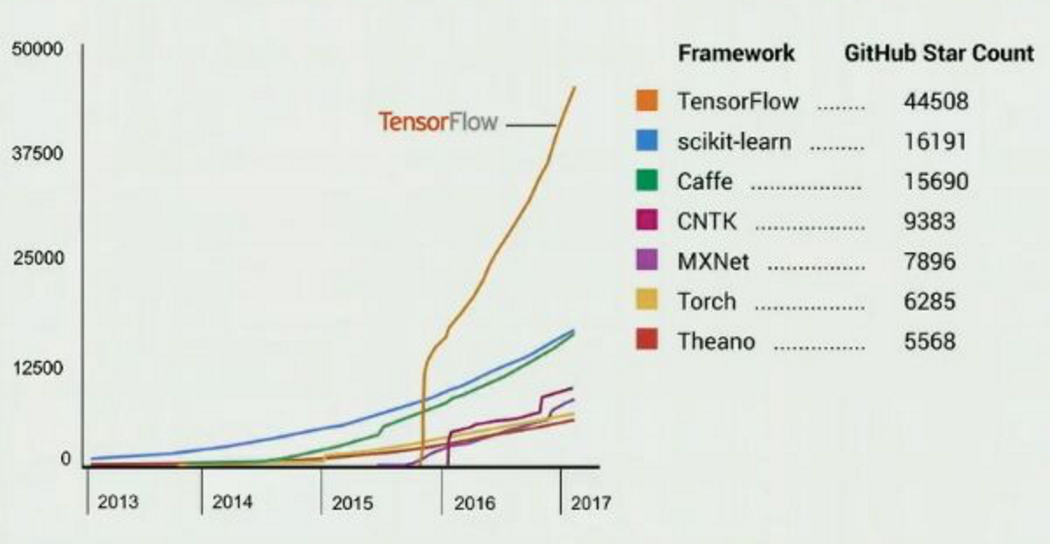
\includegraphics[width=1.0\textwidth]{figures/tf-commits.png}
\caption{TensorFlow社区活跃度}
 \label{fig:tf-commits}
\end{figure}

毫无疑问,\ascii{TensorFlow}的开源对学术界和工业界产生了巨大的影响,其极大地降低了深度学习在各个行业中应用的难度。众多的学者,工程师,企业,组织纷纷地投入到了\ascii{TensorFlow}社区,并一起完善和改进\ascii{TensorFlow},推动其不断地向前演进和发展。

\end{content}

\subsection{里程碑}

\begin{content}

\tf{}自\ascii{2015.11}开源依赖,平均一个多月发布一个版本。如\refig{tf-versions}所示,展示了\tf{}几个重要特性的发布时间。

\begin{figure}[!htbp]
\centering
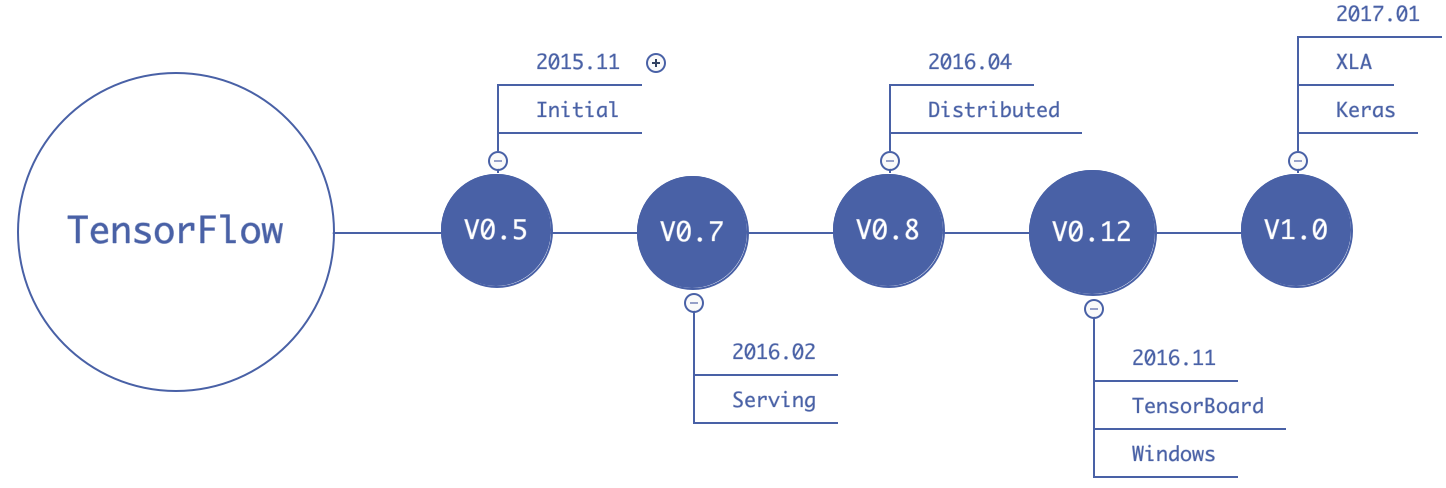
\includegraphics[width=1.0\textwidth]{figures/tf-versions.png}
\caption{TensorFlow重要里程碑}
 \label{fig:tf-versions}
\end{figure}

\end{content}

\subsection{工业应用}

\begin{content}

\ascii{TensorFlow}自开源发展一年多以来,在生产环境中被大量应用使用。在医疗方面,使用\ascii{TensorFlow}构建机器学习模型,帮助医生预测皮肤癌;在音乐、绘画领域,使用\ascii{TensorFlow}构建深度学习模型,帮助人类更好地理解艺术;在移动端,多款移动设备搭载\ascii{TensorFlow}训练的机器学习模型,用于翻译等工作。

如\refig{tf-google-apps}所示,\ascii{TensorFlow}在\ascii{Google}内部项目应用的增长也十分迅速,多个产品都有相关应用,包括:\ascii{Search, Gmail, Translate,  Maps}等等。

\begin{figure}[!htbp]
\centering
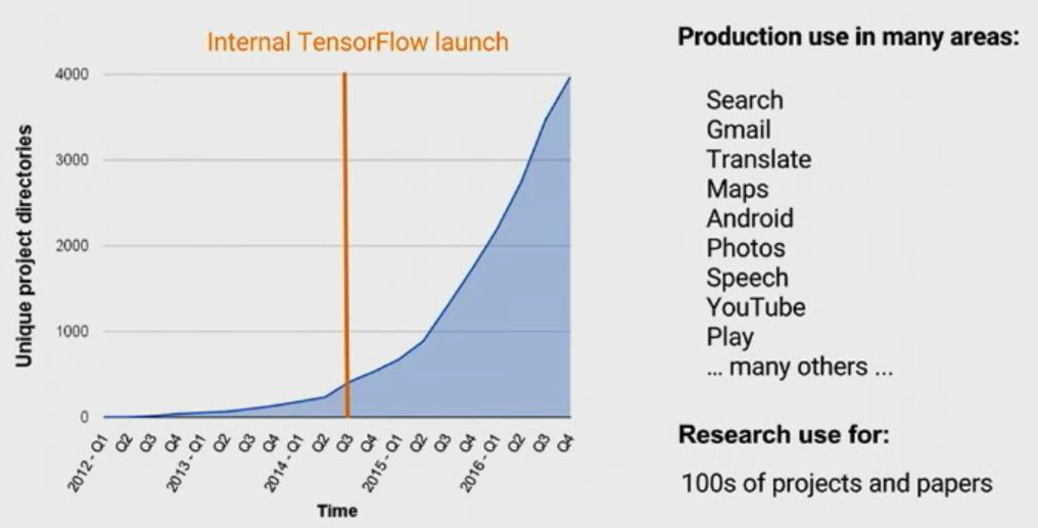
\includegraphics[width=1.0\textwidth]{figures/tf-google-apps.png}
\caption{TensorFlow在Google内部使用情况}
 \label{fig:tf-google-apps}
\end{figure}


\end{content}
\begin{savequote}[45mm]
\ascii{Any fool can write code that a computer can understand. Good programmers write code that humans can understand.}
\qauthor{\ascii{- Martin Flower}}
\end{savequote}

\chapter{系统架构} 
\label{ch:architecture}

\begin{content}

本章将阐述\tf{}的系统架构,并一个简单的例子,讲述图结构的变换过程,加深理解\tf{}运行时的工作机理。

\end{content}

\section{系统架构}

\begin{content}

\tf{}的系统结构以\ascii{C API}为界,将整个系统分为「前端」和「后端」两个子系统:

\begin{enum}
  \eitem{前端系统:提供编程模型,负责构造计算图;}
  \eitem{后端系统:提供运行时环境,负责执行计算图。} 
\end{enum}

\begin{figure}[!htbp]
\centering
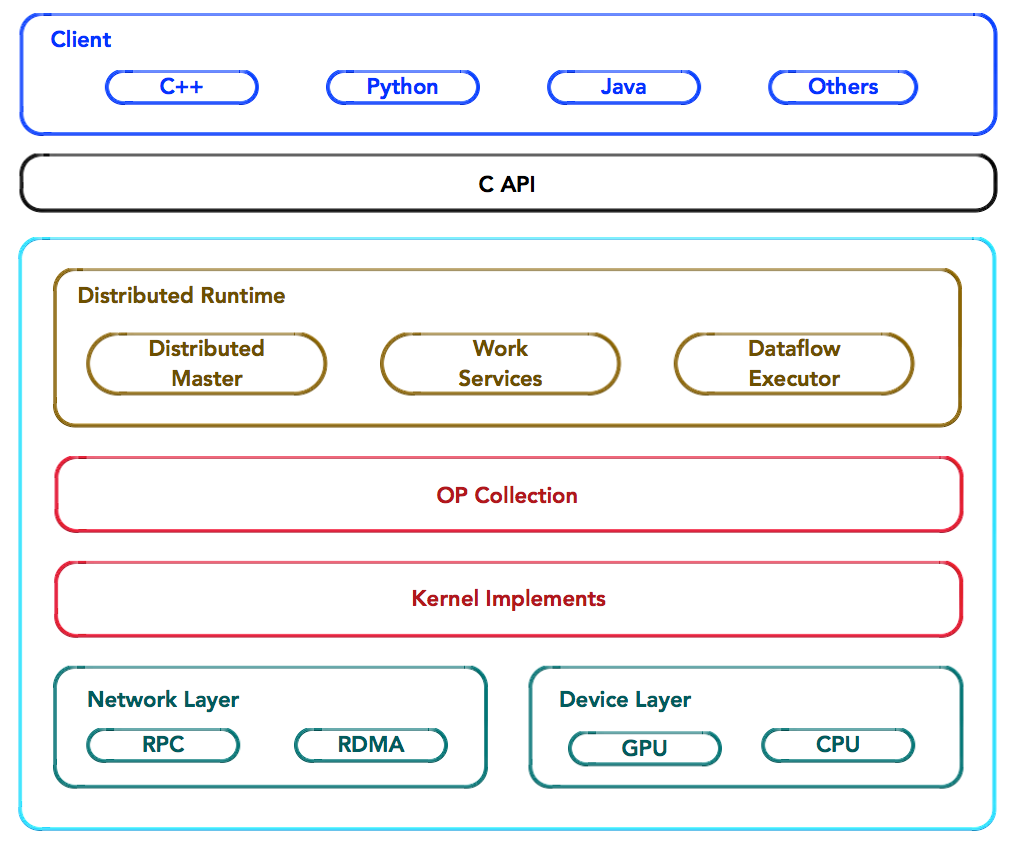
\includegraphics[width=0.9\textwidth]{figures/tf-architecture.png}
\caption{TensorFlow系统架构}
 \label{fig:tf-architecture}
\end{figure}

如\refig{tf-architecture}所示,重点关注系统中如下\ascii{4}个基本组件,它们是系统分布式运行时的核心。

\subsection{Client}

\ascii{Client}是前端系统的主要组成部分,它是一个支持多语言的编程环境。\ascii{Client}基于\ascii{TensorFlow}的编程接口,构造计算图。目前,\ascii{TensorFlow}支持\ascii{Python}和\ascii{C++}的编程接口较为完善,尤其对\ascii{Python}支持最佳;并且,对其他编程语言的编程接口的支持日益完善。

此时,\ascii{TensorFlow}并未执行任何的图计算,直至与后台计算引擎建立\ascii{Session},并以\ascii{Session}为桥梁,建立\ascii{Client}与\ascii{Master}之间的通道,将\ascii{Protobuf}格式的\ascii{GraphDef}发送至\ascii{Master},启动计算图的执行过程。

\subsection{Master}

在分布式的运行时环境中,\ascii{Client}根据\code{Session.run}传递整个计算图给后端的\ascii{Master};此时,计算图是完整的,常称为\ascii{Full Graph}。

随后,\ascii{Master}根据\ascii{Client}通过\code{Session.run}传递\code{fetches}参数列表,反向遍历\ascii{Full Graph},并按照依赖关系,对其实施剪枝,最终计算得到所依赖的「最小子图」,常称为\ascii{Client Graph}。

随后,\ascii{Master}负责将\ascii{Client Graph}按照任务的名称分裂\ascii{(split-by-task)}为多个「子图片段」,常称为\ascii{(Graph Partition)};其中,每个\ascii{Worker}对应一个\ascii{Graph Partition}。

随后,\ascii{Master}将\ascii{Graph Partition}分别注册到相应的\ascii{Worker}上,以便在不同的\ascii{Worker}上并发执行这些「子图片段」。

最后,\ascii{Master}将通知所有\ascii{Work}启动相应的\ascii{Graph Partition}的执行;其中,\ascii{Work}之间可能存在数据交互,\ascii{Master}不参与两者之间的数据交换,它们自行通信,独立交换数据即可,直至计算完成。

\subsection{Worker}

对于每以个任务,\tf{}都将启动一个\ascii{Worker}实例。\ascii{Worker}主要负责如下\ascii{3}个方面的职责:

\begin{enum}
  \eitem{处理来自\ascii{Master}的请求;}
  \eitem{调度\ascii{OP}的\ascii{Kernel}实现,执行本地子图;} 
  \eitem{协同任务之间的数据通信。}
\end{enum}

首先,\ascii{Worker}收到\ascii{Master}发送过来的图执行命令,此时的计算图相对于\ascii{Worker}是完整的,也称为\ascii{Full Graph},它对应于\ascii{Master}的一个\ascii{Graph Partition}。随后,\ascii{Worker}也会执行图剪枝,得到最小依赖的\ascii{Client Graph}。

随后,\ascii{Worker}根据当前可用的硬件环境,包括\ascii{(GPU/CPU)}资源,按照\ascii{OP}设备的约束规范,再将\ascii{Cliet Graph}分裂\ascii{(split-by-device)}为多个\ascii{Graph Partition};其中,每个计算设备对应一个\ascii{Graph Partition};随后,\ascii{Worker}启动所有当前设备的\ascii{Graph Partition}的执行。

最后,对于每一个计算设备,\ascii{Worker}将按照计算图中节点之间的依赖关系执行拓扑排序算法,并依次调用\ascii{OP}的\ascii{Kernel}实现,完成\ascii{OP}的运算(一种典型的多态实现技术)。其中,\ascii{Worker}还要负责将\ascii{OP}运算的结果发送到其他的\ascii{Work};或者接受来自其他\ascii{Worker}发送给它运算的结果,以便实现\ascii{Worker}之间的数据交互。

\subsection{Kernel}

\ascii{Kernel}是\ascii{OP}在某种硬件设备的特定实现,它负责执行\ascii{OP}的具体运算。目前,\ascii{TensorFlow}系统中包含\ascii{200}多个标准的\ascii{OP},包括数值计算,多维数组操作,控制流,状态管理等。

每一个\ascii{OP}根据设备类型都会存在一个优化了的\ascii{Kernel}实现。在运行时,运行时根据\ascii{OP}的设备约束贵方,及其本地设备的类型,为\ascii{OP}选择特定的\ascii{Kernel}实现,完成该\ascii{OP}的计算。

其中,大多数\ascii{Kernel}基于\ascii{Eigen::Tensor}实现。其中,\ascii{Eigen::Tensor}是一个使用\ascii{C++}模板技术,为多核\ascii{CPU/GPU}生成高效的并发代码。但是,\ascii{TensorFlow}也可以灵活地直接使用\ascii{cuDNN}实现更高效的\ascii{Kernel}。

此外,\ascii{TensorFlow}实现了矢量化技术,在高吞吐量、以数据为中心的应用需求中,及其移动设备中,实现更高效的推理。如果对于复合\ascii{OP}的子计算过程很难表示,或执行效率低下,\ascii{TensorFlow}甚至支持更高效的\ascii{Kernel}注册,其扩展性表现相当优越。

\end{content}

\section{图控制}

\begin{content}

随后,通过一个最简单的例子,进一步抽丝剥茧,逐渐挖掘出\tf{}计算图的控制与运行机制。


\subsection{组建集群}

如\refig{tf-1ps-1worker}所示。假如存在一个简单的分布式环境:\ascii{1 PS + 1 Worker},并将其划分为两个任务:

\begin{enum}
  \eitem{\ascii{ps0}: 使用\code{/job:ps/task:0}标记,负责模型参数的存储和更新;}
  \eitem{\ascii{worker0}: \code{/job:worker/task:0}标记,负责模型的训练。} 
\end{enum}

\begin{figure}[!htbp]
\centering
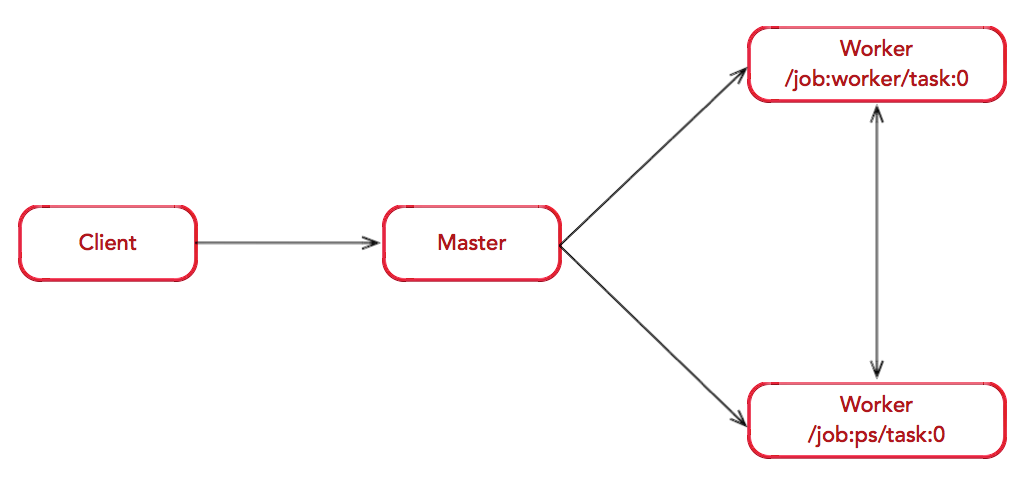
\includegraphics[width=0.9\textwidth]{figures/tf-1ps-1worker.png}
\caption{TensorFlow集群:\ascii{1 PS + 1 Worker}}
 \label{fig:tf-1ps-1worker}
\end{figure}

\subsection{图构造}

如\refig{tf-graph-construction}所示。\ascii{Client}构建了一个简单计算图;首先,将$w$与$x$进行矩阵相乘,再与截距$b$按位相加,最后更新至$s$。

\begin{figure}[!htbp]
\centering
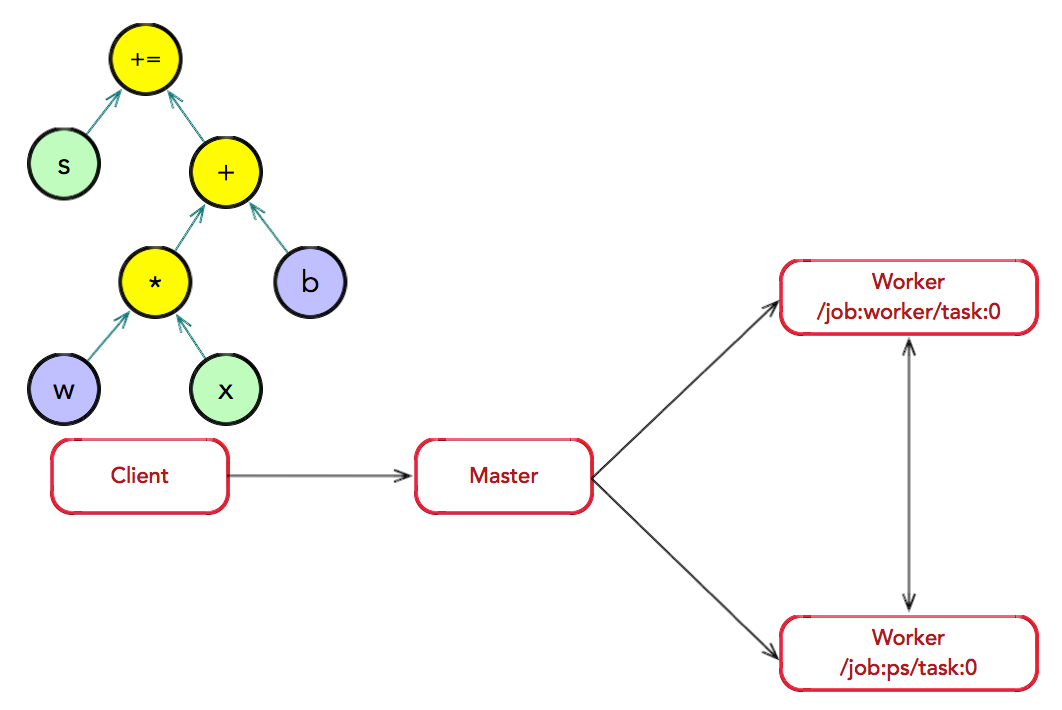
\includegraphics[width=0.9\textwidth]{figures/tf-graph-construction.png}
\caption{图构造}}
 \label{fig:tf-graph-construction}
\end{figure}

\subsection{图执行}

如\refig{tf-graph-execution}所示。首先,\ascii{Client}创建一个\code{Session}实例,建立与\ascii{Master}之间的通道;接着,\ascii{Client}通过调用\code{Sess.run}将计算图传递给\ascii{Master}。

随后,\ascii{Master}便开始启动一次\ascii{Step}的图计算过程。在执行之前,\ascii{Master}会实施一系列优化技术,例如「公共表达式消除」,「常量折叠」等。最后,\ascii{Master}负责任务之间的协同,执行优化后的计算子图。

\begin{figure}[!htbp]
\centering
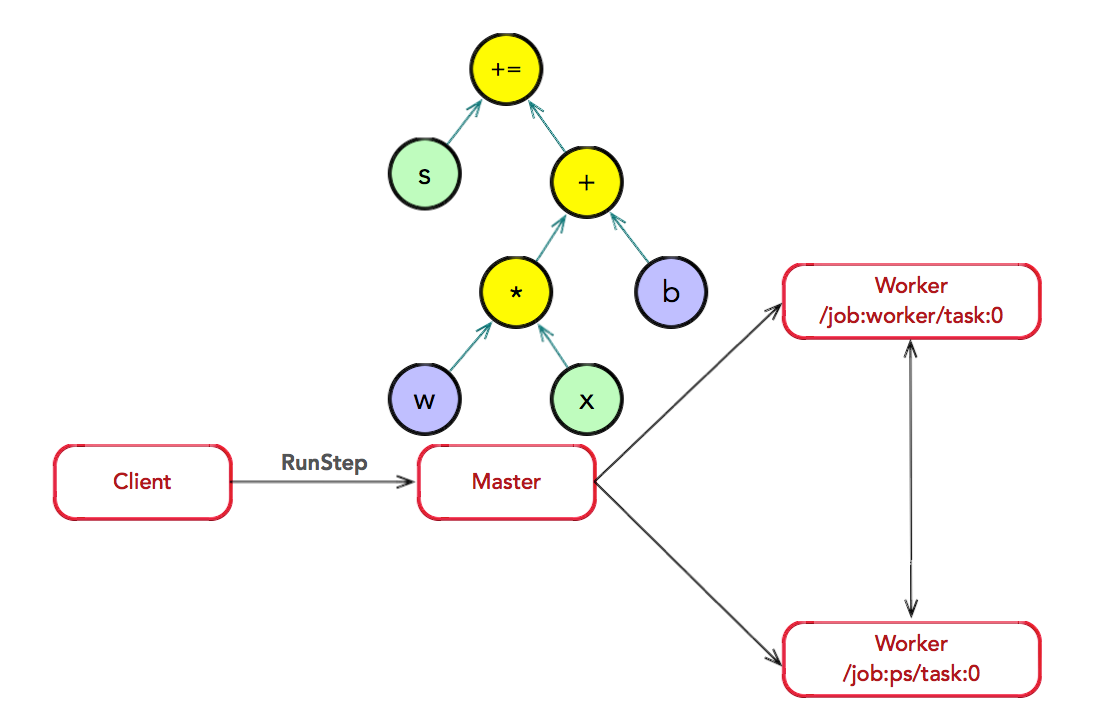
\includegraphics[width=0.9\textwidth]{figures/tf-graph-execution.png}
\caption{图执行}}
 \label{fig:tf-graph-execution}
\end{figure}

\subsubsection{图分裂}

如\refig{tf-graph-split-by-task}所示。存在一种合理的图划分算法。\ascii{Master}将模型参数相关的\ascii{OP}划分为一组,并放置在\ascii{ps0}任务上;其他\ascii{OP}划分为另外一组,放置在\ascii{worker0}任务上执行。

\begin{figure}[!htbp]
\centering
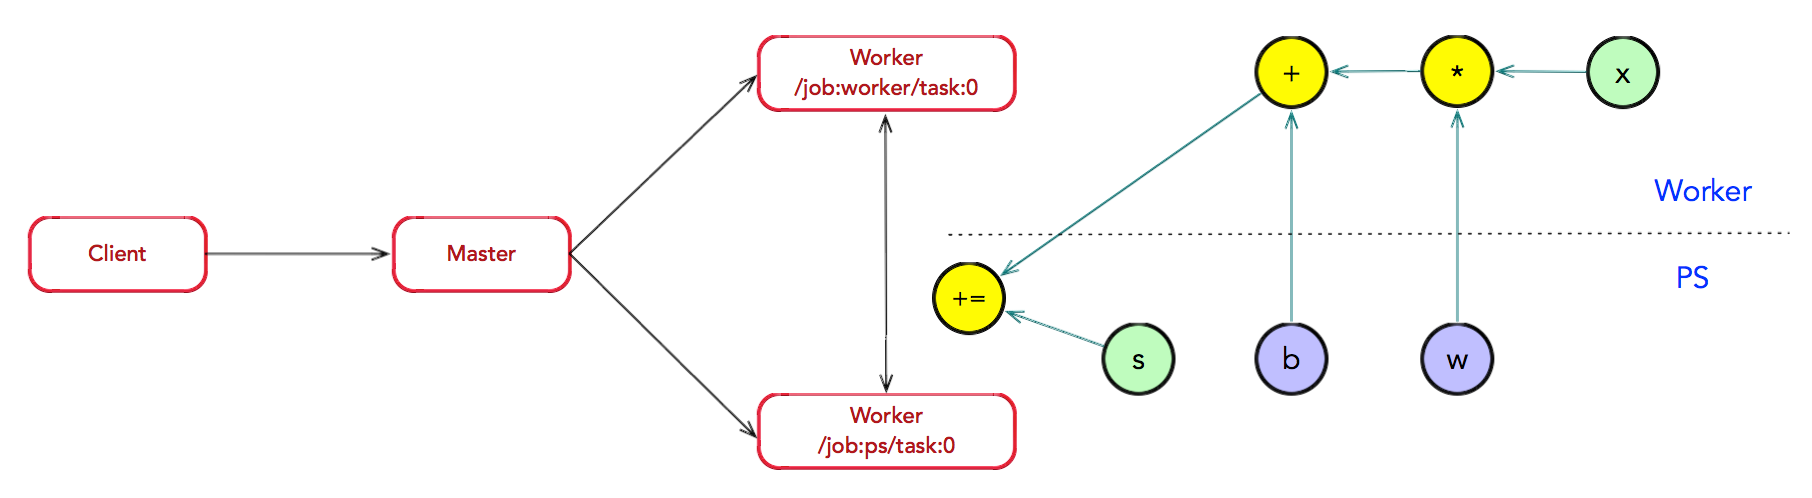
\includegraphics[width=0.9\textwidth]{figures/tf-graph-split-by-task.png}
\caption{图分裂:按任务划分}}
 \label{fig:tf-graph-split-by-task}
\end{figure}

\subsubsection{子图注册}

如\refig{tf-register-graph}所示。在图分离过程中,如果计算图的边跨越任务节点,\ascii{Master}将该边进行分裂,在两个任务之间插入\ascii{Send}和\ascii{Recv}节点,实现数据的传递。

其中,\ascii{Send}和\ascii{Recv}节点也是\ascii{OP},这是两个特殊的\ascii{OP},由内部运行时管理和控制,对用户不可见;并且,它们仅用于数据的通信,并没有任何数据计算的逻辑。

最后,\ascii{Master}通过调用\code{RegisterGraph}接口,将\ascii{Graph Partition}注册给相应的任务中,并由相应的\ascii{Worker}负责执行。

\begin{figure}[!htbp]
\centering
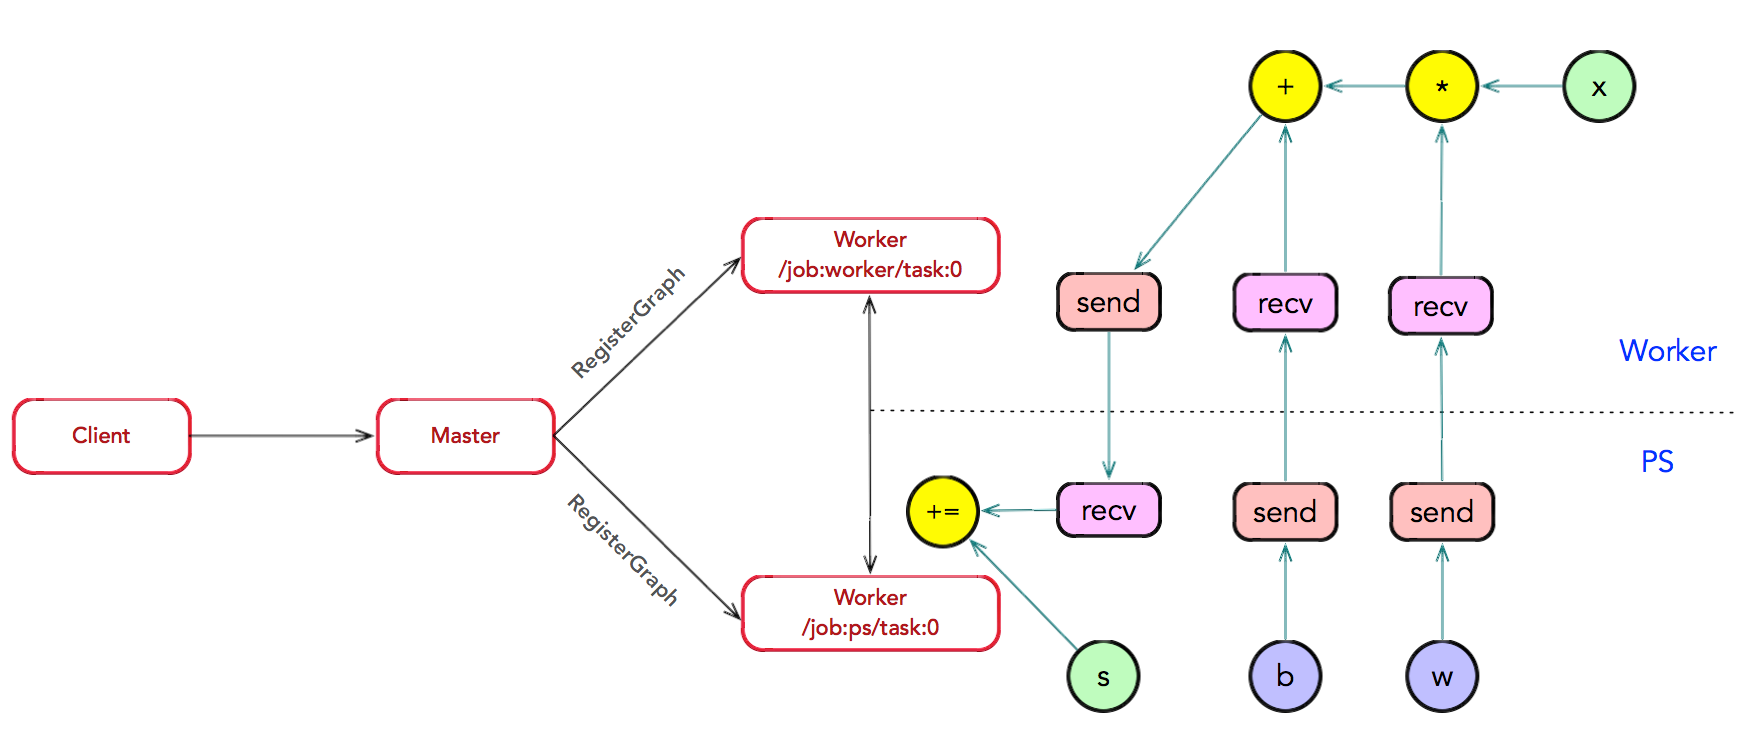
\includegraphics[width=0.9\textwidth]{figures/tf-register-graph.png}
\caption{子图注册:插入Send和Recv节点}}
 \label{fig:tf-register-graph}
\end{figure}

\subsubsection{子图运算}

如\refig{tf-run-graph}所示。\ascii{Master}通过调用\code{RunGraph}接口,通知所有\ascii{Worker}执行子图运算。其中,\ascii{Worker}之间通过调用\code{RecvTensor}接口,完成数据的交互。

\begin{figure}[!htbp]
\centering
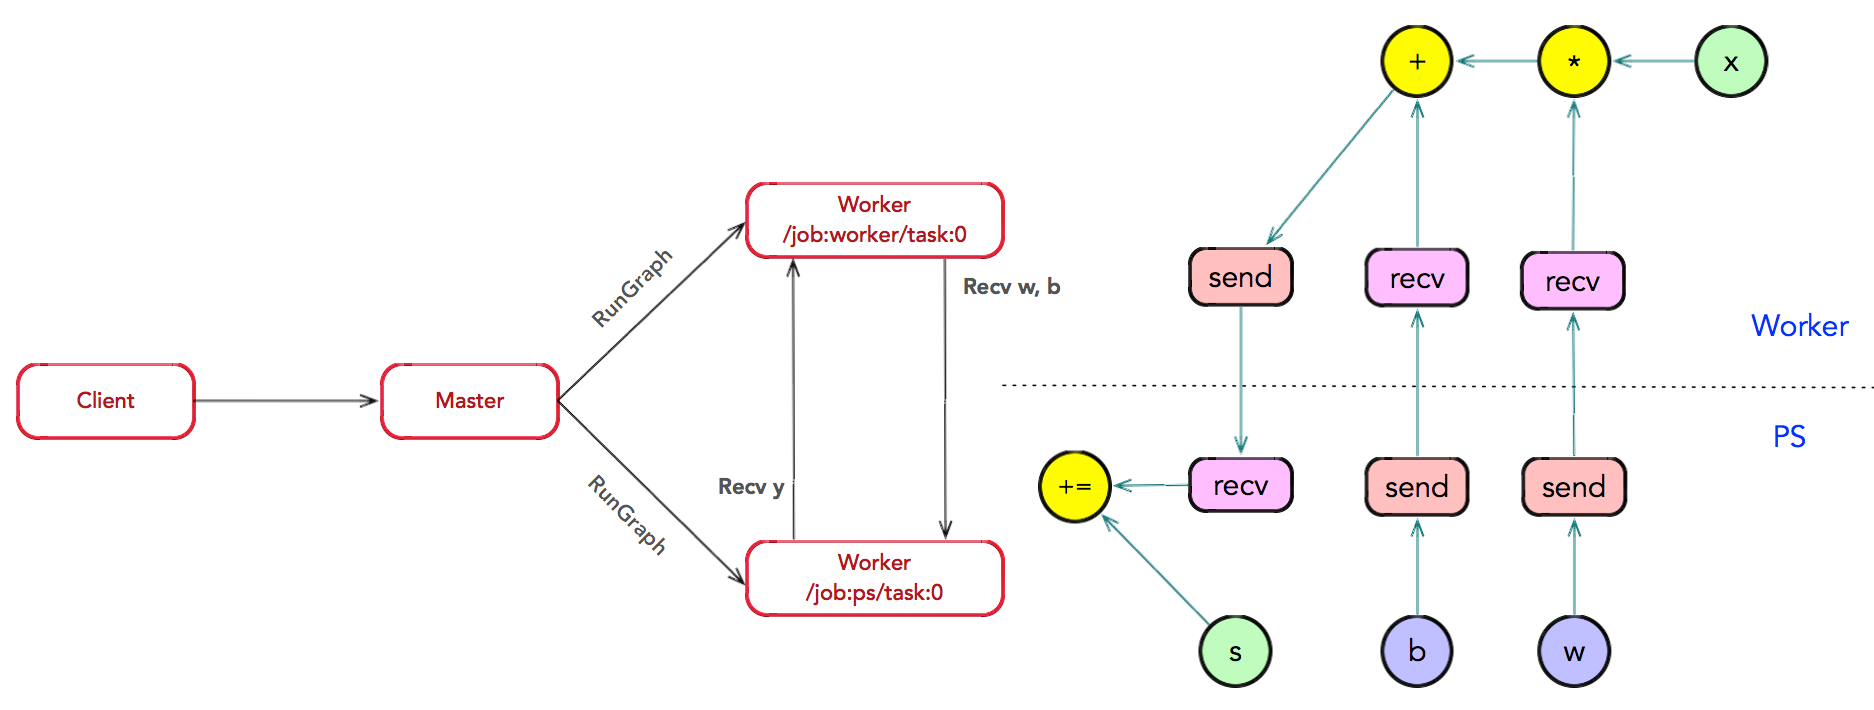
\includegraphics[width=0.9\textwidth]{figures/tf-run-graph.png}
\caption{子图执行}}
 \label{fig:tf-run-graph}
\end{figure}

\end{content}














%%%%%%%%%%%%%%%%%%%%%%
\backmatter
%\listoffigures
%\myclearpage
%\listoftables
%\myclearpage

%\include{contents/appendix}	

% %% 加入参考文献支持
% \bibliographystyle{alpha}
% \bibliography{contents/ref}

\end{document}
%%%% 正文部分结束
%%%%%%%%------------------------------------------------------------------------
